\documentclass[a4paper, 10pt]{article}
\usepackage{fancyhdr}

\pagestyle{fancy}
\fancyhead[L]{\footnotesize  APPLICATIONS OF QUANTUM CALCULUS}
\fancyhead[R]{\footnotesize  \leftmark}

\usepackage[english]{babel}
\usepackage[latin1]{inputenc}
\usepackage{empheq, amsmath, amssymb, amsthm, amssymb, indentfirst, setspace, hyperref, graphics, graphicx, verbatim, pgfplots, listings, xcolor, multicol, stmaryrd, listings, appendix}
\usepackage[super]{nth}
\usepackage[ruled, linesnumbered]{algorithm2e}
\usepackage{tikz}
\usepackage{courier}
\usepackage[nottoc]{tocbibind}

\newtheorem{theorem}{Theorem }[section]
\newtheorem{definition}{Definition }[section]

\numberwithin{equation}{section}
\numberwithin{figure}{section}
\numberwithin{table}{section}

\definecolor{mygreen}{rgb}{0,0.6,0}
\definecolor{mygray}{rgb}{0.5,0.5,0.5}
\definecolor{mymauve}{rgb}{0.58,0,0.82}

\lstset{ %
	backgroundcolor=\color{white},   % choose the background color
	basicstyle=\footnotesize\ttfamily,        % size of fonts used for the code
	breaklines=true,                 % automatic line breaking only at whitespace
	captionpos=b,                    % sets the caption-position to bottom
	commentstyle=\color{mygreen},    % comment style
	escapeinside={\%*}{*)},          % if you want to add LaTeX within your code
	keywordstyle=\color{blue},       % keyword style
	stringstyle=\color{mymauve},     % string literal style
}

%%%%%%%%%%%%%%%%%%%%%%%%%%%%%%%%%%%%%%%
%        TO DO:
% Comment Python codes
% Add results for Shor
% Finish section 6
% Write Introduction
% Write Final considerations
%%%%%%%%%%%%%%%%%%%%%%%%%%%%%%%%%%%%

\begin{document}

\begin{titlepage}
	\centering
	\begin{figure}[h!]
		\centering
		
\includegraphics[width=4cm]{Figures/cs}
	\end{figure}
	\vspace{3cm}
	{\scshape\Huge Applications of\\ Quantum Calculus:\par}
	\vspace{2mm}
	{\scshape\huge Shor's algorithm and probability distributions\par}
	\vspace{1.5cm}
	{\Large \nth{2} year Long Project\par}
	\vspace{2cm}
	{\large \textit{Students:}\\
			Ahmed BEN AISSA\\
			Elie MOKBEL\\
			Henrique MIYAMOTO\\
			Pierre MINSSEN\par}
	\vspace{1.5cm}
	{\large \textit{Supervisor:}\\
			Prof. Beno�t VALIRON \par}
	\vfill
	\large \today
\end{titlepage}

\tableofcontents

\newpage
\section{Introduction}
In 2017, thirty years after Richard Feynman, David Deutsch and other renown scientists set the first concepts and definitions of quantum computing, IBM launched the IBM Q Experience the first commercially usable quantum computer. This put forward a new horizon of possibilities regarding this ground-breaking technology \cite{medium}.

A quantum computer uses quantum mechanics principles such as superposition and entanglement to perform computation. This type of computer provides an exponential speed growth compared to classical computer.

One of the most famous quantum algorithms was developed by Peter Shor in 1994 \cite{shor}. It allows quantum computers to factorize integers exponentially quicker than the best classical algorithm. This could mean the end of the current cryptographic system that is largely based on the fact that classical algorithm takes an unrealistic amount of time to make such a factorization on large integers.

Another example of a quantum algorithm is the creation of superpositions that corresponds to efficiently integrable probability distributions.

In this report, we explore these two algorithms on more depth, with an example of an implementation and a complexity study. The document is organised as follows: Section \ref{sec:basics} is a reminder on basic concepts of quantum calculus; Section \ref{section2} presents Shor's algorithm from a theoretical point of view; Section \ref{sec:oracle} presents a construction for the oracle used in Shor's algorithm from a circuit point of view; Section \ref{sec:results} presents some results and discussions; and finally Section \ref{sec:prob} presents the problem of probability superpositions and the proposed implementation.

The material is available on GitHub \cite{git}.

\newpage
\section{Basic concepts}
\label{sec:basics}

\subsection{Qubits}
Classical computers operate on strings of bits (0 or 1) and produce other strings of bits. Classical data is supposed to be clonable, erasable, readable and not supposed to change when left untouched.

In quantum computation, on the other hand, the bits are replaced by \textit{quantum bits} or \textit{qubits}, which are unitary elements of the 2-dimensional complex Hilbert space $\mathbb{C}^2$. We choose the orthonormal basis called \textit{computational basis}
$$ |0\rangle = \begin{pmatrix} 1 \\0 \end{pmatrix} \text{ and } |1 \rangle = \begin{pmatrix} 0 \\1 \end{pmatrix}. $$

A general qubit can be seen a superposition of states $|0\rangle$ and $|1\rangle$
\begin{equation}
	|\psi\rangle = \alpha|0\rangle + \beta|1\rangle,
\end{equation}
where $\alpha,\beta\in\mathbb{C}$.

The Hilbert space $\mathbb{C}^2$ is provided with an \textit{inner product} $\langle\varphi|\psi\rangle = {|\varphi\rangle}^{\dagger}|\psi\rangle = \sum_i\overline{\varphi}_i\psi_i$, which allows one to the define the \textit{norm} of a state $\||\psi\rangle\|=\sqrt{\langle\psi|\psi\rangle}$ and \textit{orthogonality} between two states when $\langle\varphi|\psi\rangle=0$.

\subsection{Bloch sphere}
The Bloch sphere is a representation of quantum states on $S^2$. Let us consider the qubit in state $|\psi\rangle = \alpha|0\rangle + \beta|1\rangle$ and the polar representations $\alpha=|\alpha|e^{i\gamma}=\cos\frac{\theta}{2}e^{i\gamma}$ and $\beta=|\beta|e^{i(\gamma+\varphi)}=\sin\frac{\theta}{2}e^{i(\gamma+\varphi)}$. Then, we can write $|\psi\rangle=e^{i\gamma}\left(\cos\frac{\theta}{2}|0\rangle+e^{i\varphi}\sin\frac{\theta}{2}|1\rangle\right)$. Neglecting the global phase factor $e^{i\gamma}$\footnote{One reason for doing so is that this factor does not change the modulus squared of amplitudes $|\alpha|^2$ and $|\beta|^2$ \cite{portugal}.}, we have the mapping
\begin{equation}
	(\theta,\varphi) \mapsto \left(\cos\frac{\theta}{2},\ e^{i\varphi}\sin\frac{\theta}{2}\right),
\end{equation}
with $\theta\in[0\,\pi]$ and $\varphi\in[0,2\pi[$.

\begin{figure}[h!]
	\centering
	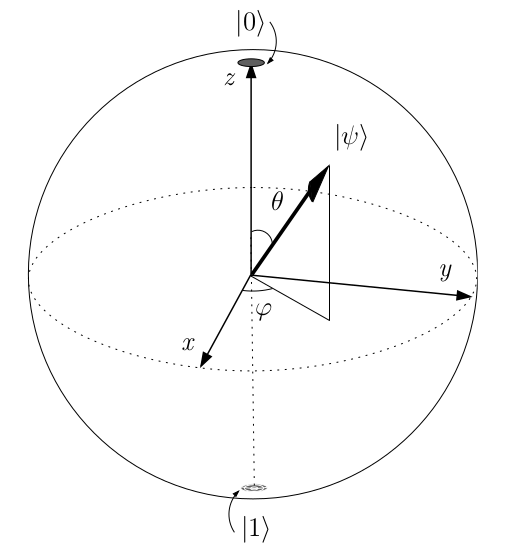
\includegraphics[width=4cm]{Figures/bloch}
	\caption{Bloch sphere \cite{portugal}.}
\end{figure}

\subsection{Measurements}
It is a probabilistic operation that allows one to recover some classical information. The measurement of $|\psi\rangle = \alpha|0\rangle + \beta|1\rangle$ returns $|0\rangle$ with probability $|\alpha|^2$ and $|1\rangle$ with probability $|\beta|^2$. It also alters the state of a qubit and forces it to collapse to state $|0\rangle$ or $|1\rangle$, respectively. In this case, we say the measurement was done against the computational basis $\{|0\rangle,|1\rangle\}$.

\subsection{Unitary operations}
The temporal evolution of an isolated quantum system is described by linear transformations, represented by matrices. Transformations that map unitary vector onto unitary vectors are called \textit{unitary transformations} $U$ and can be defined by the following property:
$$ U^{\dagger}U = UU^{\dagger} = I, $$
where $U^{\dagger} = \left(\overline{U}\right)^T$ is the adjoint matrix and $I$ is the identity. These are reversible operations. 

Some usual gates are NOT, Hadamard, phase-shift and phase-flip:

\begin{itemize}
	\item NOT
	$$ N = \begin{pmatrix}
	0 & 1\\
	1 & 0
	\end{pmatrix} $$
	\item Hadamard
	$$ H = \frac{1}{\sqrt{2}}\begin{pmatrix}
	1 & 1\\
	1 & -1
	\end{pmatrix} $$
	\item Phase-shift
	$$ V_\theta = \begin{pmatrix}
	1 & 0\\
	0 & e^{i\theta}
	\end{pmatrix} $$
	\item Phase-flip\footnote{Note that, in fact, $Z=V_\pi$.}
	$$ Z = \begin{pmatrix}
	1 & 0\\
	0 & -1
	\end{pmatrix} $$
\end{itemize}

\subsection{Tensor product}
The tensor product between two states
$$|\psi\rangle = \begin{pmatrix}
\psi_1\\
\vdots\\
\psi_m
\end{pmatrix}
\text{ and }
|\varphi\rangle = \begin{pmatrix}
\varphi_1\\
\vdots\\
\varphi_p
\end{pmatrix}$$
is computed as
$$
|\psi\rangle \otimes |\varphi\rangle = 
\begin{pmatrix}
\psi_1\varphi_1\\
\vdots\\
\psi_1\varphi_p\\
\psi_2\varphi_1\\
\vdots\\
\psi_2\varphi_p\\
\vdots\\
\psi_m\varphi_1\\
\vdots\\
\psi_m\varphi_p\\
\end{pmatrix}.
$$

In general, given two matrices $A\in\mathbb{C}^{m \times n}$ and $B\in\mathbb{C}^{p \times q}$, the tensor product is the matrix $A\otimes B\in\mathbb{C}^{mp \times nq}$ given by
\begin{equation}
	A\otimes B = \begin{pmatrix}
	a_{11}B & a_{12}B & \cdots & a_{1n}B\\
	a_{21}B & a_{22}B & \cdots & a_{2n}B\\
	\vdots & \vdots & \ddots & \vdots\\
	a_{m1}B & a_{m2}B & \cdots & a_{mn}B\\
	\end{pmatrix}
\end{equation}
where $a_{ij}$ is the $(i,j)$-element of $A$.

Given two linear transformations $A$ and $B$, we can define a new linear mapping by
\begin{equation}
	(A \otimes B)(|u\rangle \otimes |v\rangle) = A|u\rangle \otimes B|v\rangle. 
\end{equation}

Notation:
\begin{itemize}
	\item We can indistinguishably write $|\psi\rangle \otimes |\varphi\rangle = |\psi\rangle|\varphi\rangle = |\psi,\varphi\rangle = |\psi\varphi\rangle$.
	\item $|\psi\rangle^{\otimes n} = \underbrace{|\psi\rangle \otimes \cdots |\psi\rangle}_{n \text{ times}}$ and $A^{\otimes n} = \underbrace{A \otimes \cdots A}_{n \text{ times}}$.
\end{itemize}


\subsection{Many qubits systems}

The state of a 2-qubit is an element of the tensor product space $\mathbb{C}^4 = \mathbb{C}^2 \otimes \mathbb{C}^2$, which is spanned by
$$|00\rangle = \begin{pmatrix}1\\0\\0\\0\end{pmatrix},\quad |10\rangle = \begin{pmatrix}0\\1\\0\\0\end{pmatrix},\quad |01\rangle = \begin{pmatrix}0\\0\\1\\0\end{pmatrix},\quad |11\rangle = \begin{pmatrix}0\\0\\0\\1\end{pmatrix}.$$

A generic state of 2 qubits it therefore of the form
$$ |\psi\rangle = \alpha|00\rangle + \beta|01\rangle + \gamma|10\rangle + \delta|11\rangle $$
with $|\alpha|^2+|\beta|^2+|\gamma|^2+|\delta|^2=1$.

In general, writing states as the decimal number correspoding to the binary representation (e.g. $|11\rangle \rightarrow |3\rangle$), a $n$-qubit state is described as
$$ |\psi\rangle = \sum_{i=0}^{2^n-1}\alpha_i|i\rangle, \text{ with } \sum_{i=0}^{2^n-1}|\alpha_i|^2=1. $$

As a generalisation of the 1-qubit case, the measurement of a $n$-qubit state changes it and forces it to collapse to one of the possible $|i\rangle$ states, each of which is measured with probability $|\alpha_i|^2$.

Among unitary operations available to 2-qubits states, we have the swap gate $X$ and the control-not gate $N_C$:
$$ X = \begin{pmatrix}
1 & 0 & 0 & 0\\
0 & 0 & 1 & 0\\
0 & 1 & 0 & 0\\
0 & 0 & 0 & 1\\
\end{pmatrix},\quad
N_C = \begin{pmatrix}
1 & 0 & 0 & 0\\
0 & 1 & 0 & 0\\
0 & 0 & 0 & 1\\
0 & 0 & 1 & 0\\
\end{pmatrix}. $$

The control-not gate changes the state of the second qubit only if the first qubit is in the state $|1\rangle$. It implements the mapping $|xy\rangle \mapsto |x\rangle \otimes |x\oplus y\rangle$.

The Toffoli gate acts on 3 qubits and is a ``control-control-not'': it implements the function $|xyz\rangle \mapsto |xy\rangle \otimes |z\oplus xy\rangle$, i.e., it changes the state of the last qubit if the two first qubits are in state $|11\rangle$.

\subsection{Quantum entanglement}

Consider the states $|\psi\rangle = a|0\rangle + b|1\rangle$ and $|\varphi\rangle = c|0\rangle + d|1\rangle$. Their tensor product is $|\psi\varphi\rangle = ac|00\rangle + ad|01\rangle + bc|10\rangle + bd|11\rangle$. It turns out that a general state is not on this form, unless it has $\alpha\delta = \beta\gamma$.

We say a quantum state is \textit{entangled} when it cannot be written as a tensor product of two other states. For example, $\frac{1}{\sqrt{2}}(|00\rangle+|11\rangle)$ cannot have such a decomposition, and hence is an entangled state.

\subsection{Quantum circuits}

Quantum circuits are graphical representations of a procedure, i.e., a sequence of logical operations performed on a system. Unlike classical circuits, the wires must not be regarded as physical connections and their components are not available ``on the shelf''.

\begin{figure}[h!]
	\centering
	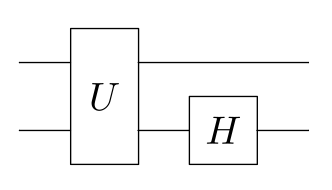
\includegraphics[width=4cm]{Figures/circuit}
	\caption{Example of quantum circuit representing $|\psi\rangle \mapsto (I\otimes H)(U|\psi\rangle)$ \cite{valiron}.}
\end{figure}

\newpage
\section{Shor's algorithm}
\label{section2}

The advantage of quantum algorithms over classical ones appears when using some quantum property such as entanglement or the interference, brought by complex coefficients.

In fact, quantum algorithms are based on a few ``real'' quantum constructions, such as quantum Fourier transform, quantum walk and amplitude amplification. The rest is composed of classical analysis and possibly an \textit{oracle}: a quantum circuit corresponding to a reversible operation.

Some interesting problems in algebra and number theory reduce to the problem of order finding. For example, the problem of factorising an integer number, which is addressed by Shor's algorithm \cite{shor}.

\subsection{Factorisation}

The objective of the \textit{factorisation problem} is to factorise a big number $N$ into prime numbers. Note that at least $n=\lceil\log_2N\rceil$ qubits are needed to store $N$ and that $n$ is the maximum number of prime factors. We will show how this problem reduces to the problem of finding the order of a randomly generated integer $x<N$.

If $N$ is even, 2 is trivially a factor. In addition, if $x$ and $N$ have common factors, then $\gcd(x,N)$ gives a factor of $N$; so we focus on investigating the case when $x$ and $N$ are coprimes.

\begin{definition}
	The order of $x$ modulo $N$ is the least positive integer $r$ such that
	\begin{equation}
		x^r \equiv 1 \mod N.
	\end{equation}
\end{definition}

\begin{theorem}[Euler's Theorem]
	If $x$ and $N$ are coprime positive integers, then
	\begin{equation}
		x^{\varphi(N)} \equiv 1 \mod N,
	\end{equation}
	where $\varphi(N)$ is the Euler's totient function, i.e., it indicates the number of coprimes to $N$ which are less or equal to it.
\end{theorem}

The \textit{order finding problem} is to find $r$, given $x$ and $N$ coprimes. The algorithm is built up on the following two theorems.

\begin{theorem}
	Let $N$ be a composite number stored with $n$ qubits and $x$ be non-trivial solution of the equation $x^2 \equiv 1 \mod N$ in the range $1 \le x \le N$, i.e., $x \not\equiv \pm 1 \mod N$. Then at least one of $\gcd(x+1,N)$ and $\gcd(x-1,N)$ is a non-trivial factor of $N$.
\end{theorem}

\begin{proof}
	Note that $x^2 \equiv 1 \mod N \Leftrightarrow x^2-1 \equiv 0 \mod N \Leftrightarrow (x+1)(x-1) \equiv 0 \mod N$, which means that $N$ is a divisor of $(x+1)(x-1)$. If $1<x<N-1$, then $0<x-1<x+1<N$ and $N$ cannot be a divisor of $(x+1)$ neither of $(x-1)$ separately. So both $(x+1)$ and $(x-1)$ must have factors of $N$. In this case, at least one of $\gcd(x+1,N)$ and $\gcd(x-1,N)$ produce a non-trivial factor of $N$\footnote{Such factor can be computed by using Euclid's algorithm.}.
\end{proof}

\begin{theorem}
	Suppose $N = p_{1}^{\alpha_1}...p_{m}^{\alpha_m}$ is the prime factorisation of and odd composite positive integer. Let $x$ be an integer chose uniformly at random such that $1 \le x\le N-1$ and $\gcd(x,N)=1$. Let $r$ be the order of $x$ modulo $N$. Then
	\begin{equation}
		\mathrm{Pr}\{\text{$r$ is even and $x^{r/2}\not\equiv\pm1\mod N$}\} \ge 1-\frac{1}{2^m}.
	\end{equation}
\end{theorem}

\begin{proof}
	See \cite{ekert}, pp. 751-752\footnote{Actually, these authors use a slightly different bound for the probability: $1-1/2^{m-1}$.}.
\end{proof}

The algorithm runs as follows.

\begin{algorithm}[h!]
	\caption{Shor's algorithm for factorising $N$.}
	If $N$ is even, return the factor 2.\\
	Randomly choose $x$ such that $1 \le x \le N-1$.\\
	If $\gcd(x,N)\neq1$, return the factor $\gcd(x,N)$.\\
	Find the order $r$ of $x$ modulo $N$.\\
	If $r$ is even and $x^{r/2}\not\equiv\pm 1\mod N$, then $\gcd(x^{r/2}+1,N)$ and $\gcd(x^{r/2}-1,N)$ are non-trivial factors.\\
	Else, restart the algorithm.
\end{algorithm}

Some remarks:

\begin{itemize}
	\item The method fails if $N$ is the power of a prime number. But in this case there exists a a classical algorithm to solve the problem \cite{portugal}. %Which one?
	\item The problem is finding the order of $x$ modulo $N$, for which there is no efficient classical procedure available. This problem is addressed in the next part.
\end{itemize}

\subsection{Order finding}

The problem of order finding, i.e., given $x$ and $N$ coprimes, to find $r$ such that $x^r \equiv 1 \mod N$ is related to the matrix eigendecomposition. A unitary $U$, being a Hermitian matrix, can be decomposed as
\begin{equation}
	U=\sum_j \lambda_ju_ju_j^\dagger,
\end{equation}
where $u_j$ are orthonormal eigenvectors and $\lambda_j$ are the associated eigenvalues.

Let us assume that $N=2^n$ and consider the operation $U_x$ on $n$ qubits that implements the mapping
\begin{equation}
	U_x : \quad |j\rangle \mapsto |j\cdot x\mod N\rangle.
\end{equation}
The operator is unitary because $x$ and $N$ are coprimes and the image of $\{0,...,N-1\}$ is the whole set. In particular, $U_x^k$ sends $|j\rangle \mapsto |j\cdot x^k \mod N\rangle$, so if $x^r \equiv 1 \mod N$, the map $U_x^r$ is the identity map.

The eigenstates of $U$ are of the \footnote{To simplify notation, hereafter we shall denote $U_x$ by $U$ simply.}
\begin{equation}
	|u_s\rangle = \frac{1}{\sqrt{r}} \sum_{k=0}^{r-1}\exp{\left(-\frac{2\pi i sk}{r}\right)}|x^k \mod N \rangle
\end{equation}
for $0 \le s \le r-1$. The eigenvalues are the $r$-th roots of the unity, having the form $e^{2\pi is/r}$, since
\begin{equation}
	U|u_s\rangle = \exp\left(\frac{2\pi is}{r}\right)|u_s\rangle.
\end{equation}

An algorithm for finding such eigenvalues should be enough to find the order $r$ of $x$ modulo $N$\footnote{An alternative unitary could have been used: $V|j\rangle|k\rangle=|j\rangle|k+x^j\mod N\rangle$.}.

\subsection{Quantum Fourier transform}

The Fourier transform is an operation that can be performed faster in quantum computers. The quantum Fourier transform (QFT) \cite{griffighs} is defined in analogy with the discrete Fourier transform. It is the linear mapping:
\begin{align}
	\hat{f}\ :\ \mathbb{C}^N &\rightarrow \mathbb{C}^N \nonumber \\
	|j\rangle &\mapsto \frac{1}{\sqrt{N}}\sum_{k=0}^{N-1}e^{2\pi ijk/N}|k\rangle
\end{align}

Let us consider $N=2^n$ with orthonormal basis $\{|0\rangle,\dots,|2^n-1\rangle\}$. We shall use the \textit{binary representation} $j =: j_1j_2\dots j_n$ to represent $j = \sum_{i=1}^{n}j_{i}2^{n-i}$ and the \textit{binary fraction} $j =: 0.j_1j_2\dots j_n$ to represent $j = \sum_{i=1}^{n}j_{i}2^{-i}$.

It will be useful to consider an alternative form of the QFT which is indeed so important that could be considered its definition itself:
\begin{equation}
	|j_1\dots j_n\rangle \mapsto \frac{\left(|0\rangle+e^{2\pi i0.j_n}|1\rangle\right)\otimes\left(|0\rangle+e^{2\pi i0.j_{n-1}j_n}|1\rangle\right)\otimes\dots\otimes\left(|0\rangle+e^{2\pi i0.j_1\dots j_n}|1\rangle\right)}{2^{n/2}}.
\end{equation}

The equivalence between the two expressions can be shown as follows \cite{nielsen}:

\begin{align*}
	&\frac{1}{2^{n/2}}\sum_{k=0}^{2^n-1}e^{2\pi ijk/2^n}|k\rangle\\
	=\ &\frac{1}{2^{n/2}}\sum_{k_1=0}^{1}\dots\sum_{k_n=0}^{1}e^{2\pi ij(\sum_{l=1}^{n}k_l/2^{l})}|k_1\dots k_n\rangle \ &\text{(write in binary representation)}\\
	=\ &\frac{1}{2^{n/2}}\sum_{k_1=0}^{1}\dots\sum_{k_n=0}^{1}\prod_{l=1}^{n}\otimes e^{2\pi ijk_l/2^l}|k_l\rangle\ &\text{(tensor product decomposition)}\\
	=\ &\frac{1}{2^{n/2}}\prod_{l=1}^{n}\otimes\left( \sum_{k_l=0}^{1} e^{2\pi ijk_l/2^l}|k_l\rangle \right)\ &\text{(factorise the binary powers)}\\
	=\ &\frac{1}{2^{n/2}}\prod_{l=1}^{n}\otimes\left( |0\rangle + e^{2\pi ij/2^l} |1\rangle \right).
\end{align*}

The product representation allows one to implement the quantum circuit for the QFT using Hadamard and $R_k$ rotation gates, the latter being of the form\footnote{The attentive reader will notice that $R_k = V_{2\pi/2^k}$.}
\begin{equation}
	R_k := \begin{pmatrix}1 & 0\\ 0 & e^{2\pi i/2^k}\end{pmatrix}.
\end{equation}

\begin{figure}[h!]
	\centering
	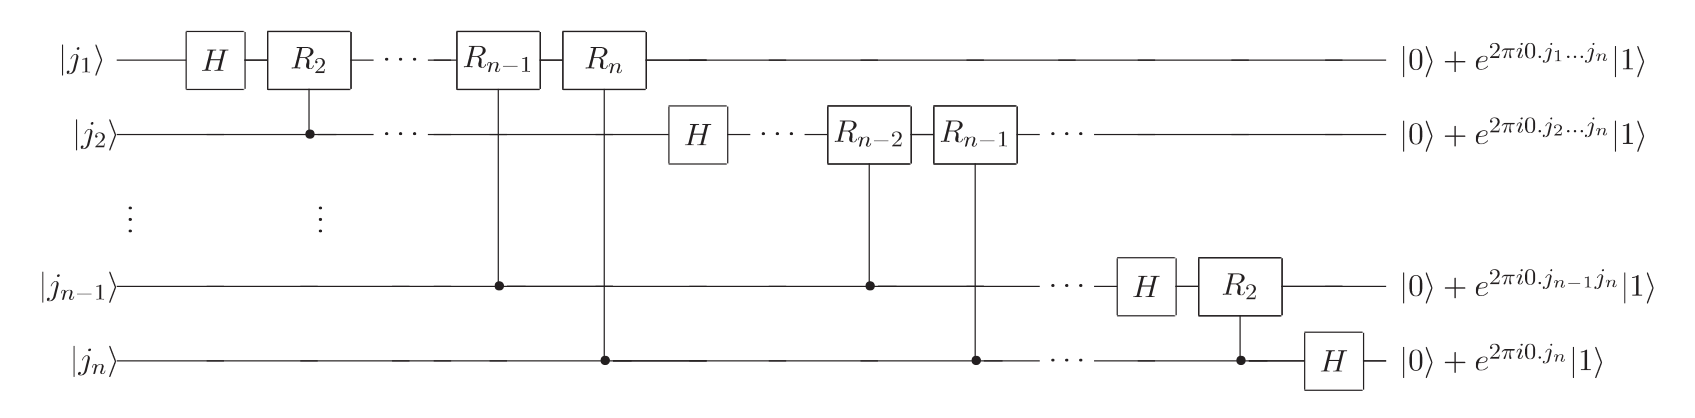
\includegraphics[width=12cm]{Figures/qft-circuit}
	\caption{Quantum circuit that implements the QFT \cite{nielsen}.}
	\label{fig-qft}
\end{figure}

To conclude this section, we remark that the QFT, as a linear operation, may be written in matrix form\cite{wiki}:

\begin{equation}
	 F = \frac{1}{\sqrt{N}}
	\begin{pmatrix}
	1 & 1 & 1 & 1 & \cdots & 1 \\
	1 & \omega_n & \omega_n^2 & \omega_n^3 & \cdots & \omega_n^{N-1} \\
	1&\omega_n^2&\omega_n^4&\omega_n^6&\cdots&\omega_n^{2(N-1)}\\ 1&\omega_n^3&\omega_n^6&\omega_n^9&\cdots&\omega_n^{3(N-1)}\\
	\vdots&\vdots&\vdots&\vdots&\ddots&\vdots\\
	1&\omega_n^{N-1}&\omega_n^{2(N-1)}&\omega_n^{3(N-1)}&\cdots&\omega_n^{(N-1)(N-1)}
	\end{pmatrix}
\end{equation}
where $N=2^n$ and $\omega_n:=e^{2\pi i/2^n}$. This allows one to verify that $FF^{\dagger} = F^{\dagger}F = I$, therefore concluding that the Fourier transform is a unitary transformation.

\subsection{Quantum phase estimation}

Suppose a unitary operator $U$ has an eigenvector $|u\rangle$ with eigenvalue $e^{2\pi i\varphi}$, where $\varphi$ is unknown. The objective of the \textit{phase estimation subroutine} is to estimate the value of $\varphi$. We assume we have oracles capable of preparing the state $|u\rangle$ and performing controlled-$U^{2^j}$ operations.

The procedure uses two registers: the first contains $t$ qubits initially in state $|0\rangle$. The number $t$ depends on the desired accuracy for $\varphi$ and on the probability we want the procedure to be successful. The second register begins with the state $|u\rangle$ and contains as many qubits as necessary to store it.

The first step is to apply the following circuit to the registers.

\begin{figure}[h!]
	\centering
	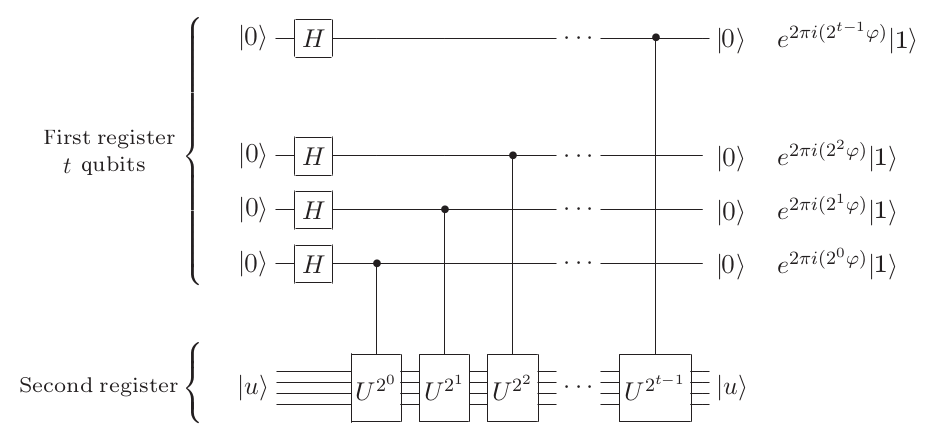
\includegraphics[width=10cm]{Figures/phase-estimation-1}
	\caption{Quantum circuit for first step of phase estimation (normalisation has been omitted on the right side) \cite{nielsen}.}
\end{figure}

The final state of the first register is
\begin{align*}
	&\frac{1}{2^{t/2}}\left(|0\rangle+e^{2\pi i2^{t-1}\varphi}|1\rangle\right)\left(|0\rangle+e^{2\pi i2^{t-2}\varphi}|1\rangle\right) \dots \left(|0\rangle+e^{2\pi i2^{0}\varphi}|1\rangle\right)\\
	=\ &\frac{1}{2^{t/2}}\sum_{k=0}^{2^t-1}e^{2\pi i\varphi k}|k\rangle.
\end{align*}

The second step is to apply the inverse Fourier transform on the first register\footnote{To do so, we just have to invert the circuit for QFT on Figure \ref{fig-qft}.} and the third step is to measure it. Note that, if we write the previous expression using the binary fraction representation, we have
$$ \frac{1}{2^{t/2}}\left(|0\rangle+e^{2\pi i0.\varphi_t}|1\rangle\right)\left(|0\rangle+e^{2\pi i0.\varphi_{t-1}\varphi_{t}}|1\rangle\right) \dots \left(|0\rangle+e^{2\pi i0.\varphi_1...\varphi_t}|1\rangle\right). $$
Comparing it with the (product) expression for the Fourier transform, one can see that the result of applying the inverse Fourier transform is the state $|\varphi_1\dots\varphi_r\rangle$ and a measurement in the computational basis gives exactly an estimation for $\varphi$!

\begin{figure}[h!]
	\centering
	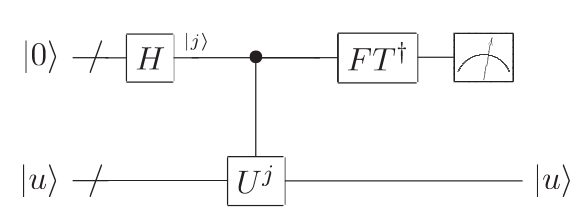
\includegraphics[width=6cm]{Figures/phase-estimation-2}
	\caption{Schematic of the overall phase estimation subroutine \cite{nielsen} .}
\end{figure}

Summarising, the phase estimation subroutine gives an estimation $\tilde{\varphi}$ to the phase of an eigenvalue of a unitary $U$, which is precisely what we wanted to implement the order finding algorithm. The inverse Fourier transform performs
$$ \frac{1}{2^{t/2}}\sum_{j=0}^{2^{t-1}}e^{2\pi i\varphi j}|j\rangle|u\rangle \mapsto |\tilde{\varphi}\rangle|u\rangle. $$

\begin{theorem}[Accuracy of $\varphi$ \cite{nielsen}, pp. 223-224]
	To successfully obtain $\varphi$ accurate to $n$ bits with probability of success at least $1-\epsilon$, we choose
	\begin{equation}
		t = n + \left\lceil \log\left(2+\frac{1}{2\epsilon}\right) \right\rceil.
	\end{equation}
\end{theorem}

\subsection{Continued fraction expansion}

Let us recapitulate what we have so far: we have reduced the factorisation problem to the order finding problem, which can be solved by calculating eigenvalues of a unitary $U$ of the form $e^{2\pi is/r}$. The quantum phase estimation procedure uses the QFT to estimate the phase $\varphi$ of an eigenvalue $e^{2\pi i\varphi}$. So we have an estimation
$$ \tilde{\varphi} \approx \frac{s}{r}. $$

It misses one building block in order to solve our problem: how to retrieve $r$ from $\tilde{\varphi}$. To do so, we shall use \textit{continued fraction expansions}. The results on this topic can be deepened in \cite{hardy}. 

\begin{definition}
	A finite simple continued fraction is an expression of the form
	\begin{equation}
		a_0 + \dfrac{1}{a_1 + \dfrac{1}{a_2 + \dfrac{1}{\ddots+\dfrac{1}{a_N}}}}
	\end{equation}
	which is denoted by $[a_0,  a_1, a_2, \cdots, a_N]$, with $a_i \in \mathbb{N}^*\ \forall i\in \llbracket 1, N\rrbracket$.\\
	We define the $n$-th convergent to this continued fraction as $[a_0,\dots,a_n]$ for $0\le n \le N$.
\end{definition}

\begin{theorem}
	The $n$-th convergent may be written as a fraction
	\begin{equation}
		[a_0,\dots,a_n]=\frac{p_n}{q_n}
	\end{equation}
	whose coefficients are given by the following recurrence relation:
	$$
	\begin{array}{ll}
		p_0:=a_0\\
		q_0:=1
	\end{array}\quad
	\begin{array}{ll}
		p_1:=a_1a_0+1\\
		q_1:=a
	\end{array}\quad
	\begin{array}{ll}
		p_n:=a_np_{n-1}+p_{n-2}\\
		q_n:=a_nq_{n-1}+q_{n-2}
	\end{array}\ (2\le n \le N).
	$$
\end{theorem}

\begin{proof}
	See \cite{hardy}, pp. 166-167.
\end{proof}

The next two theorems will present the \textit{continued fractions algorithm} to approximate $\tilde{\varphi}$ by a $n$-th convergent and explain why it suffices to solve our problem.

\begin{theorem}[Continued fraction algorithm]
	Any rational number $x$ can be represented by a finite simple continued fraction $[a_0,\dots,a_N]$.\\
\end{theorem}

\begin{proof}
	See \cite{hardy}, pp. 173-174.
\end{proof}

The algorithm runs as follows.

\begin{algorithm}[h!]
	\caption{Continued fraction algorithm for rational $x$.}
	Set $a_0 = \lfloor x \rfloor$. Then $x=a_0+\xi_0$, with $\xi_0\in[0,1[$.\\
	While $\xi_i \neq 0$: $a_{i+1}=\lfloor1/\xi_{i}\rfloor$ and $1/\xi_{i}=a_{i+1}+\xi_{i+1}$, with $\xi_{i+1}\in[0,1[$.\\
	The continued fraction is $[a_0,\dots,a_N]$, where $N$ is such that $\xi_N=0$.
\end{algorithm}

\begin{theorem}
	Suppose $s/r$ is a rational number such that
	\begin{equation}
		\left|\frac{s}{r}-\varphi\right| \le \frac{1}{2r^2}.
	\end{equation}
	Then $s/r$ is a convergent of the continued fraction for $\varphi$.
\end{theorem}

\begin{proof}
	See \cite{hardy}, pp. 196-197.
\end{proof}

Since $\tilde{\varphi}$ is an approximation of $s/r$ accurate to $n=\lceil\log_2N\rceil$ qubits, the theorem applies. Summarising, given $\tilde{\varphi}$, we can use the continued fraction algorithm to find an irreducible fraction $s'/r'=s/r$. Then, $r'$ is our candidate for the order. We check calculating $x^{r'} \mod N$; if the result is $1$, we are done!

\newpage
\section{Oracle circuit}
\label{sec:oracle}

Now that we know the quantum algorithm to factorise a number, we can devote our attention to the implementation in terms of quantum circuit. Although we have already provided a circuit for the QFT, the oracle remains a mysterious black box. In this Section, we show how it can be implemented. In \cite{beauregard}, the author presents a circuit implementation that aims to reduce the number of qubits needed, while using a polynomial number of elementary quantum gates.

\subsection{Adder gate}

An initial version for the adder circuit is presented by \cite{draper}. Instead of basing on classical circuits which use at least $3n$ qubits to sum two $n$-qubits number, by composing carry gates and sum gates, the author presents an implementation based on the QFT. The idea, in order to sum $a$ and $b$, is to compute the Quantum Fourier transform of $a$, $\phi(a)$, and then use $b$ to compute $\phi(a+b)$. The inverse QFT is then applied to recover the desired result.

Using the following notation\footnote{Here, understand $e\left(\frac{1}{2^k}\right)$ as $\exp\left(\frac{2\pi i}{2^k}\right)$.} to conditional rotation gates $R_k$, it is possible to describe the adder circuit as in Figure \ref{fig-adder}.

\begin{figure}[h!]
	\centering
	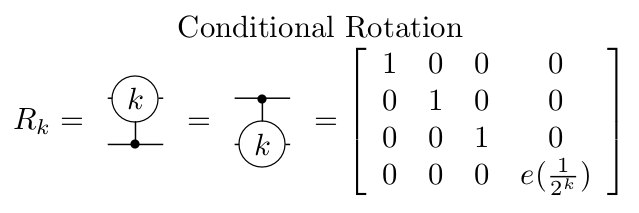
\includegraphics[width=6cm]{Figures/rotation-k}
\end{figure}

\begin{figure}[h!]
	\centering
	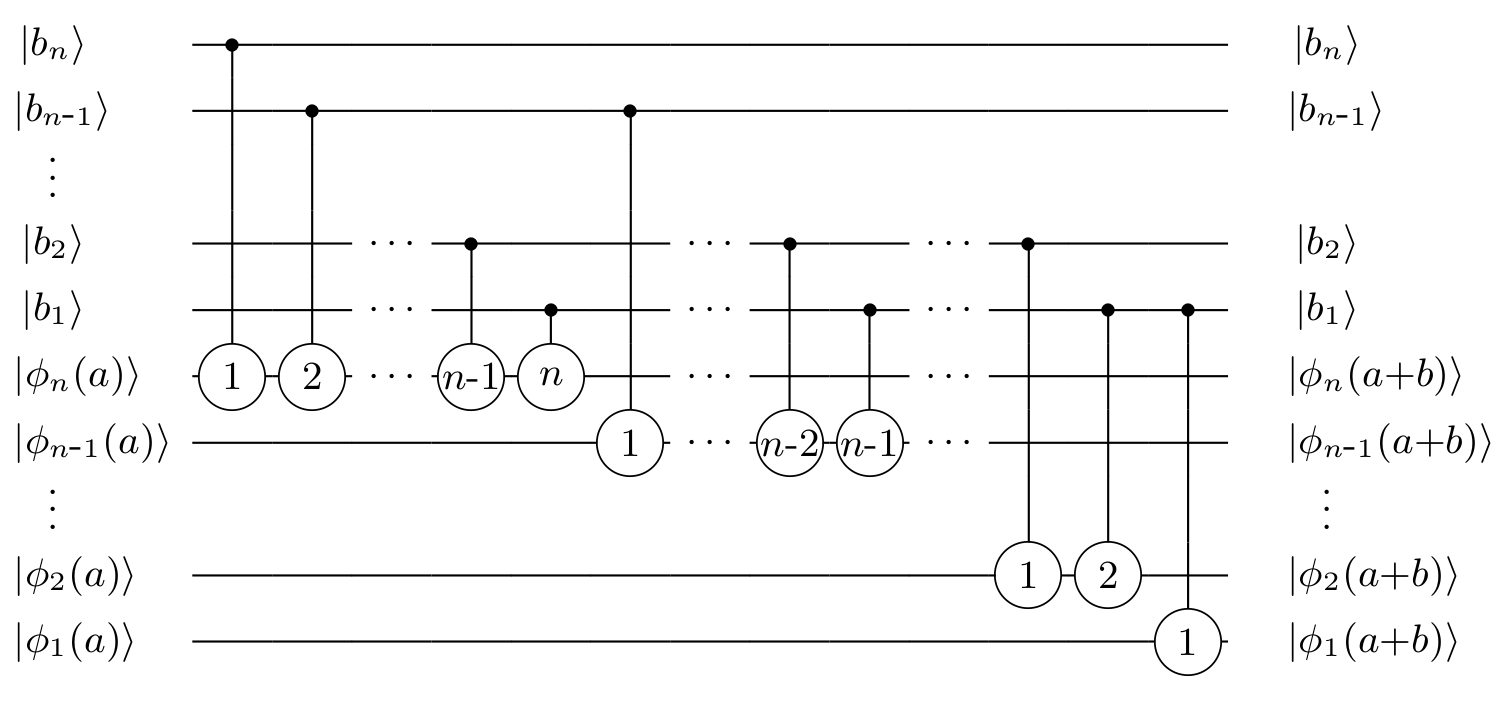
\includegraphics[width=10cm]{Figures/adder1}
	\caption{Quantum adder based on QFT, as presented in \cite{draper}. The QFT operator is denoted $\phi(\cdot)$.}
	\label{fig-adder}
\end{figure}

The advantage of this method is that a quantum computer that can perform simultaneous calculations can decrease the time of execution, for instance, by executing all depth 1 rotations simultaneously, and then all depth 2 rotations and so on. In particular, in the case of using the Approximate Quantum Fourier Transform (AQFT)\footnote{This technique consists in reducing the rotations blocks as $k$ gets large, as for large values of $k$, the rotation block approaches an identity gate ($R_k \approx I$). The optimal value of $k$ is around $\log_2n$ \cite{draper}.}, this quantum addition can be computed in $n\log_2n$ operations.

To follow what happens in this circuit, we shall resume the notation introduced in the presentation of the QFT (\S \ref{section2}).

\begin{align*}
	|\phi_n(a)\rangle &\rightarrow \frac{1}{\sqrt{2}}\left(|0\rangle+e^{2\pi i(0.a_na_{n-1}\cdots a_1+0.b_n)}|1\rangle\right)\quad&\text{($R_1$ rotation from $b_n$)}\\
					  &\rightarrow \frac{1}{\sqrt{2}}\left(|0\rangle+e^{2\pi i(0.a_na_{n-1}\cdots a_1+0.b_nb_{n-1})}|1\rangle\right)\quad&\text{($R_2$ rotation from $b_{n-1}$)}\\
					  &\qquad \vdots\\
					  &\rightarrow \frac{1}{\sqrt{2}}\left(|0\rangle+e^{2\pi i(0.a_na_{n-1}\cdots a_1+0.b_nb_{n-1}\cdots b_1)}|1\rangle\right)\quad&\text{($R_n$ rotation from $b_1$)}\\
					  & = |\phi(a+b)\rangle.
\end{align*}

A slight variation of the implementation presented so far is introduced by \cite{beauregard}, with the notation $\phi$-ADD($a$). As he points out, the objective of implementing this sum is to afterwards be able to retrieve the order modulo $N$ of $a$ (which plays the role of $x$ in the previous notation). Thus, $a$ is classical and the qubits that represent it may be replaced by classical bits. An additional qubit is added to prevent overflow.

\begin{figure}[h!]
	\centering
	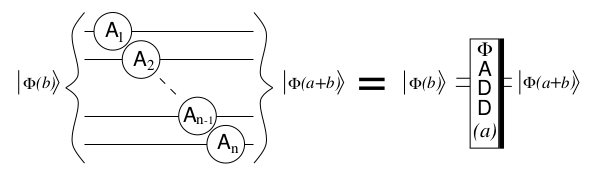
\includegraphics[width=8cm]{Figures/adder2}
	\caption{Circuit of $\phi$-adder as presented in \cite{beauregard}.}
\end{figure}

The reverse of this gate (denoted with the thick bar on the left) will be used to subtraction and comparison.

\begin{figure}[h!]
	\centering
	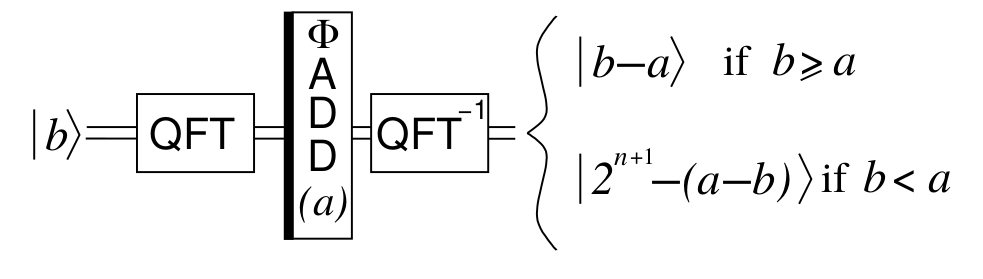
\includegraphics[width=6cm]{Figures/adder3}
	\caption{Circuit of reverse $\phi$-ADD$(a)$ \cite{beauregard}.}
\end{figure}

\subsection{Modular adder gate}

The goal now is to use the $\phi$-ADD$(a)$ to build a adder modulo $N$. This means that we have to subtract $N$ from the result if $a+b \ge N$. We will denote this block $\phi$-ADD$(a)$-mod-$N$. The whole block is controlled by two qubits.

The circuit operation, depicted in Figure \ref{fig-modadd} is described as follows:

\begin{itemize}
	\item The circuit begins with $|\phi(b)\rangle$ as input.
	\item After the $\phi$-ADD$(a)$ block, the value in the register is $\phi(a+b)$ (with no overflow, assuming there is an extra $|0\rangle$ qubit in $|b\rangle$).
	\item Then, we apply a reverse $\phi$-ADD$N$, having $\phi(a+b-N)$ on the register. We apply this operation even without knowing if it was really necessary to subtract $N$ from the previous result.
	\item Now we have to check if this operation was indeed necessary or not. But to access the most significant bit of it, we have to pass the whole value through an inverse QFT gate. The most significant bit is used to control a CNOT gate on the ancilla qubit $|0\rangle$.
	\item The QFT is reapplied, so we come back to $\phi(a+b-N)$.
	\item The value $N$ is added back if the subtraction was unnecessary, so that $a+b < N$. The value in the register is now $\phi(a+b)\mod N$.
	\item Close to being satisfied, we just have to restore the ancilla to assure that our gate corresponds to a reversible operation. The trick is to note that $(a+b)\mod N \Leftrightarrow a+b<N$. So one can apply a circuit analogous to the previous one: subtract $a$, recover the most significant qubit of the result (which will be $|0\rangle$), invert it and use it on controlled-not over the ancilla, which will be restored to $|0\rangle$; at the end, restore $a$.
\end{itemize}

\begin{figure}[h!]
	\centering
	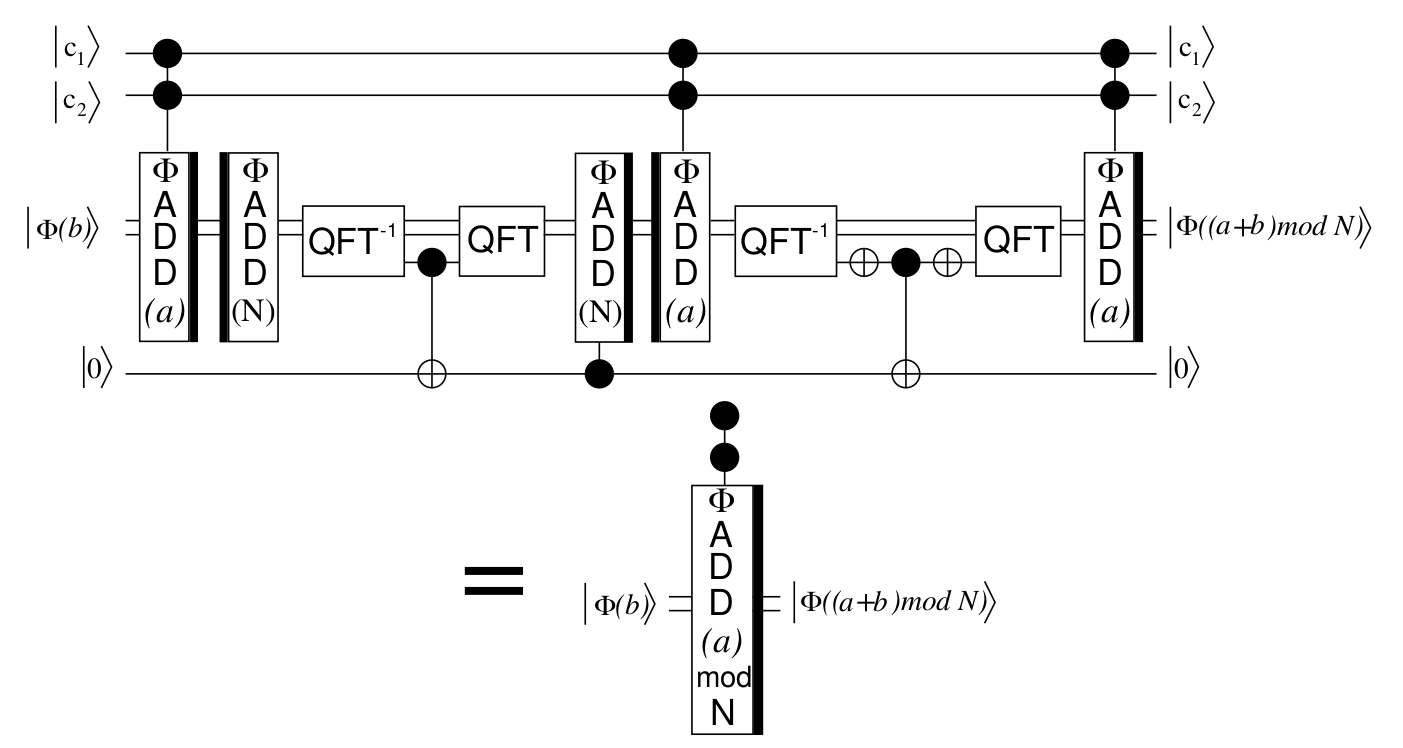
\includegraphics[width=9cm]{Figures/modadder}
	\caption{Circuit of $\phi$-adder modulo $N$ as presented in \cite{beauregard}.}
	\label{fig-modadd}
\end{figure}

\subsection{Controlled multiplier gate}

Now, we can use the previous $\phi$-ADD$(a)$-mod-$N$ to build a controlled multiplied gate, denoted CMULT$(a)$-mod-$N$. This gate has input $|c\rangle|x\rangle|b\rangle$ and is to compute $|c\rangle|x\rangle|(b+ax)\mod N\rangle$ if $|c\rangle=|1\rangle$, or not to alter any qubit otherwise.

The implementation with $\phi$-ADD$(a)$-mod-$N$ is based on the fact that
\begin{equation}
	(ax) \mod N = \sum_{i=0}^{n-1}2^{i}ax_i \mod N
\end{equation}
where the modulo $N$ has to be applied on each step of the summation. Thus all we need are $n$ successive $\phi$-ADD$(2^i a)$-mod-$N$ gates.

\begin{figure}[h!]
	\centering
	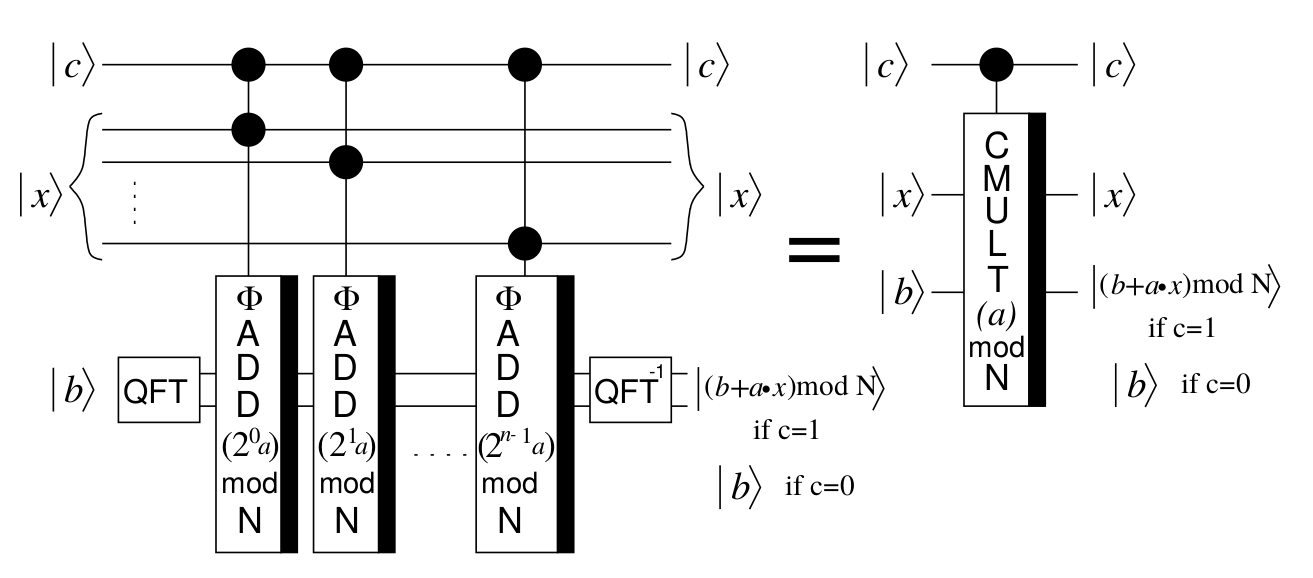
\includegraphics[width=8cm]{Figures/cmult}
	\caption{Circuit of CMULT$(a)$-mod-$N$ as presented in \cite{beauregard}.}
	\label{fig-cmult}
\end{figure}

\subsection{Controlled $U$ gate}

In the previous step, we got a controlled gate that implements the mapping $|x\rangle|b\rangle \mapsto |x\rangle|b+(ax)\mod N\rangle$. However, in fact, we would like to implement $|x\rangle \mapsto |x\rangle|(ax)\mod N\rangle$, which corresponds to our $U$-gate unitary operation. The implementation is presented in Figure \ref{fig-ugate}.

Let us follow the steps of the circuit:
\begin{itemize}
	\item Start by applying the CMULT$(a)$-mod-$N$ gate to the input $|c\rangle|x\rangle|0\rangle$.
	\item Apply a controlled-SWAP gate (controlled by $|c\rangle$ as well). Indeed, it is only necessary to apply it on $n$ qubits, because the most significant one of $(ax) \mod N$ will always be $|0\rangle$ (to store the overflow of the $\phi$-adder).
	\item Then, apply the inverse CMULT$(a^{-1})$-mod-$N$\footnote{The inverse modulo $N$ of $a$, $a^{-1}$, can be computed via Euclid's algorithm.}.
\end{itemize}

The sequence of performed operations is

\begin{multline*}
|x\rangle|0\rangle \rightarrow |x\rangle|(ax)\mod N\rangle \rightarrow |(ax)\mod N\rangle|x\rangle \rightarrow\\
|(ax)\mod N\rangle|x-a^{-1}ax\rangle = |(ax)\mod N\rangle|0\rangle.
\end{multline*}

As a result, the controlled-$U$ gate implements $|x\rangle|0\rangle \mapsto |(ax) \mod N\rangle|0\rangle$. To compute a $(\text{control}-U_a)^n$, it is enough to apply $\text{control}-U_{a^n}$ instead of applying the same gate multiple times.

\begin{figure}[h!]
	\centering
	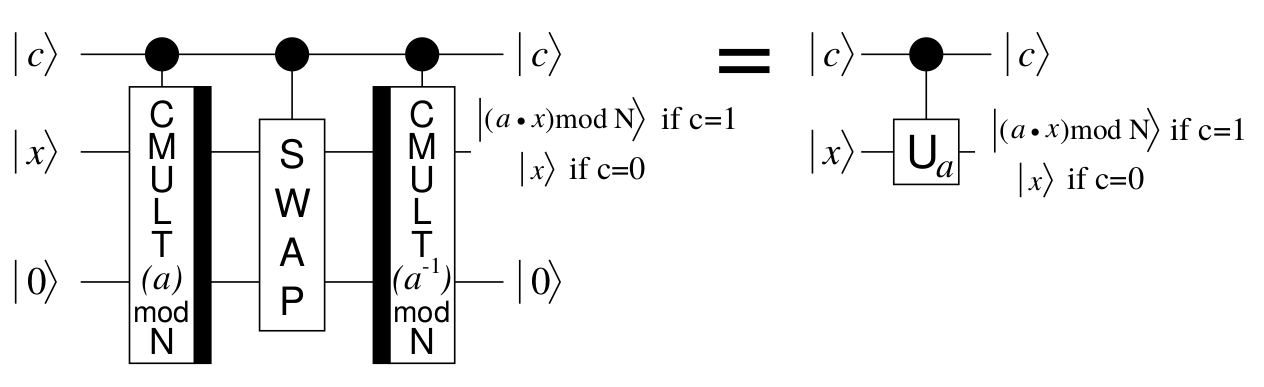
\includegraphics[width=8cm]{Figures/ugate}
	\caption{Circuit of controlled $U$-gate as presented in \cite{beauregard}.}
	\label{fig-ugate}
\end{figure}

\clearpage
\newpage
\section{Results and discussion}
\label{sec:results}

The implementations were made in Python using \textit{ProjectQ}, which is an open-source software framework for quantum computing \cite{projectq, steiger}. We remember our codes are available on GitHub \cite{git}.

The following subsections present results and discussions on that implementation.

\subsection{Circuits}

The quantum circuit for factorisation implements Shor's algorithm as described in \S\ref{section2} using the oracle as described in \S\ref{sec:oracle}. ProjectQ has a feature that generates circuits as \LaTeX\ images. Although the complete circuit and more complex blocks easily become too big to be presented here, some simpler blocks are showed in Figures \ref{fig:gen1}, \ref{fig:gen2}, \ref{fig:gen3}.

\begin{figure}[h!]
	\centering
	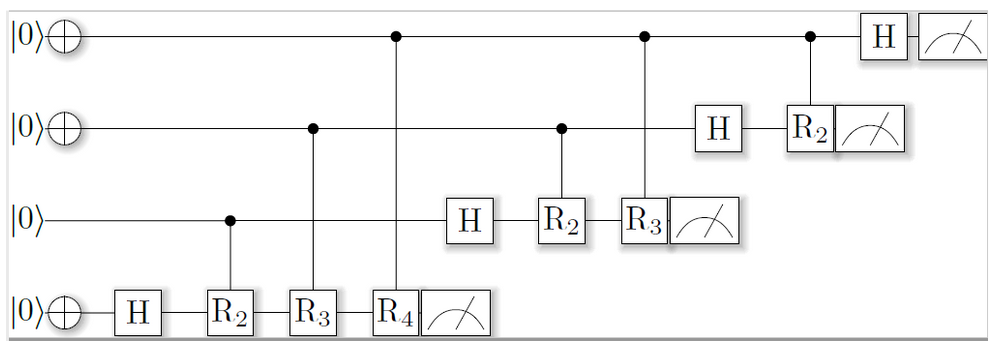
\includegraphics[width=8cm]{Figures/generated-qft}
	\caption{Circuit example for the QFT with 4 qubits.}
	\label{fig:gen1}
\end{figure}

\begin{figure}[h!]
	\centering
	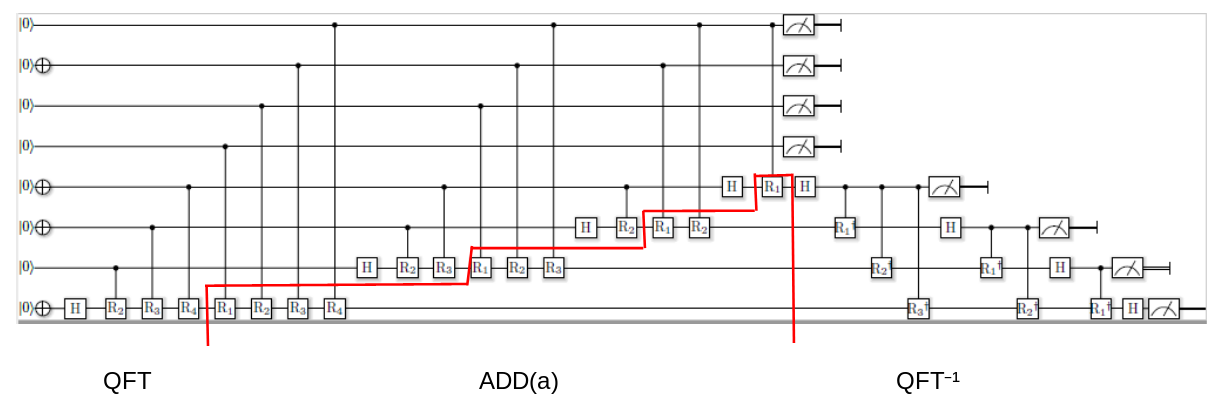
\includegraphics[width=10cm]{Figures/generated-adder}
	\caption{Circuit for the adder block, with possible overflow.}
	\label{fig:gen2}
\end{figure}

\begin{figure}[h!]
	\centering
	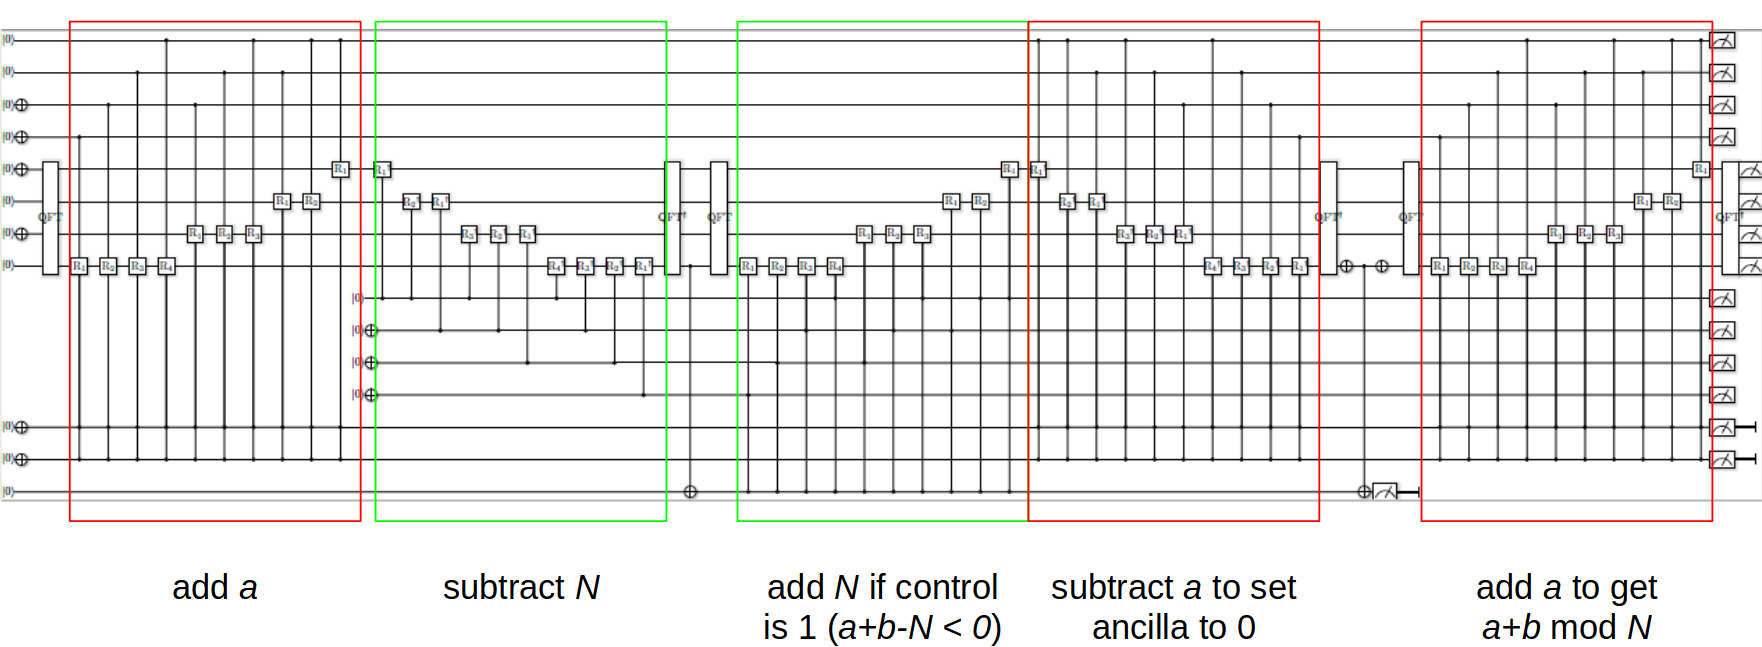
\includegraphics[width=12cm]{Figures/generated-modadder}
	\caption{Circuit for modular adder block.}
	\label{fig:gen3}
\end{figure}

\subsection{Complexity Analysis}
\label{sec:complexity}

A complexity analysis is performed by \cite{beauregard}, presenting number of qubits, order of number of gates and order of depth for each part of the circuit proposed by them (cf. \S \ref{sec:oracle}) to factorise an integer $N$ stored with $n=\lceil\log_2N\rceil$ bits. The results are summarised in Table \ref{table-complexity}.

\begin{table}[h!]
	\centering
	\caption{Complexity analysis of circuit parts \cite{beauregard}.}
		\label{table-complexity}
		\begin{tabular}{|c|c|c|c|}
			\hline
			Circuit            		 & Number of qubits & Order of gates & Order of depth \\ \hline
			$\phi$-ADD$(a)$          & $n+1$            & $O(n)$         & $O(1)$         \\ 
			$\phi$-ADD$(a)$-mod-$N$  & $n+4$            & $O(nk_{\max})$   & $O(n)$         \\ 
			CMULT$(a)$-mod-$N$    	 & $2n+3$           & $O(n^2k_{\max})$ & $O(n^2)$       \\ 
			$U_a$ gate            	 & $2n+3$           & $O(n^2k_{\max})$ & $O(n^2)$       \\ 
			Shor                  	 & $2n+3$           & $O(n^3k_{\max})$ & $O(n^3)$       \\ \hline
		\end{tabular}
		When using the exact QFT, $k_{\max}=n$.
\end{table}

We have compared the number of gates of some of the circuits we have implemented with the result proposed above. Using MATLAB, we fitted each set of data to a polynomial function of the respective degree (Table \ref{table-results}, Figures \ref{fit-cmult}, \ref{fit-ua}, \ref{fit-shor}). Note that, having used used the exact QFT approach in our implementation, $k_{\max}=n$\footnote{This relation can be reduced with the approximate QFT technique up to $k_{\max}=O(\log(n/\epsilon))$, for any $\epsilon$ polynomial in $1/n$ \cite{beauregard}.}. We have performed tests for $N=2^{k}-1,\quad k\in\llbracket 3, 19\rrbracket$ and we counted the swap gates $X$ used for qubits initialisation in the total number of gates.

\begin{table}[h!]
	\centering
	\caption{Order of number of gates and fitting polynomials in $n$.}
	\label{table-results}
	\begin{tabular}{|c|c|c|}
		\hline
		Circuit            & Order & Fitting polynomial\\ \hline
		CMULT$(a)$-mod-$N$ & $O(n^3)$ & $2.5\ n^3 + 7.5\ n^2 + 18\ n + 11$ 							 \\ 
		$U_a$ gate         & $O(n^3)$ & $5\ n^3 + 15\ n^2 + 32\ n + 12$       						 \\
		Shor               & $O(n^4)$ & $10\ n^4 + 26\ n^2 - 16\ n + 2$    \\ \hline
	\end{tabular}
\end{table}

\begin{figure}[h!]
	\centering
	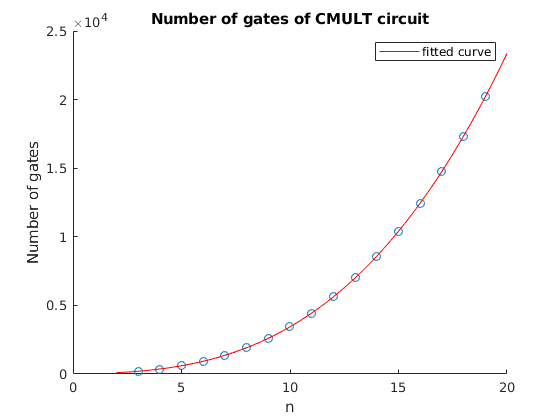
\includegraphics[width=7cm]{Figures/data-cmult}
	\caption{Number of gates of CMULT$(a)$-mod-$N$ circuit as function of $n$.}
	\label{fit-cmult}
\end{figure}

\begin{figure}[h!]
	\centering
	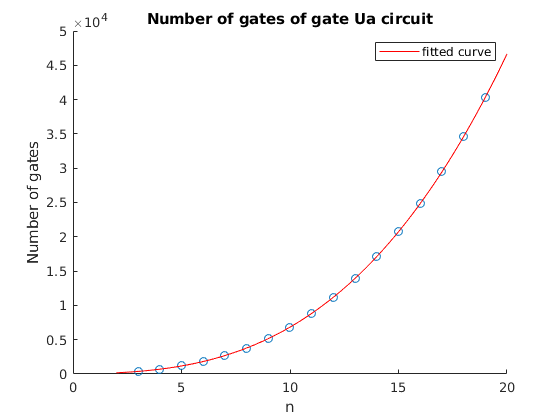
\includegraphics[width=7cm]{Figures/data-Ua}
	\caption{Number of gates of $U_a$ gate circuit as function of $n$.}
	\label{fit-ua}
\end{figure}

\begin{figure}[h!]
	\centering
	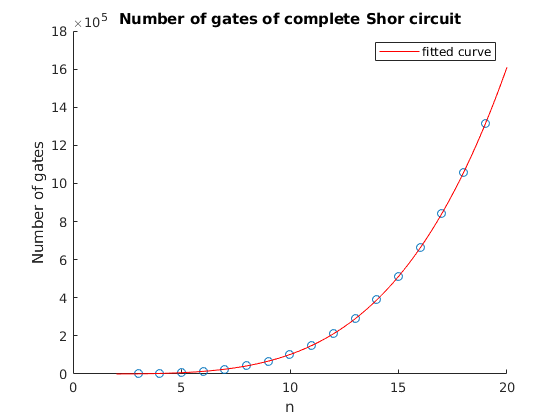
\includegraphics[width=7cm]{Figures/data-shor}
	\caption{Number of gates of Shor's algorithm circuit as function of $n$.}
	\label{fit-shor}
\end{figure}

We observe that all resulting polynomials fit well the sets of data, matching the theoretical results in Table \ref{table-complexity}.

\subsection{Discussion}

Although we are able to successfully factorise integer numbers, we find limitations to run Shor's algorithm with big numbers because of the low capacities of our PC\footnote{We use a 4GB PC with AMD A9-9420 Radeon 3.00 GHz.}. The largest number we have been able to (non-trivially) factorise was $21=3\times7$. Even if we use the C++ simulator (instead of the Python one) of ProjectQ to improve the testing, we are able to use 5 qubits of entry at best. The running of the algorithm in full-capacity shall wait further development of a quantum computer.

\clearpage
\newpage
\section{Probability superpositions}
\label{sec:prob}

After successfully implementing Shor's algorithm, we devoted our attention to the problem of creating quantum superpositions that correspond to efficiently integrable probability distributions, as presented in the paper \textit{Creating superpositions that correspond to efficiently integrable probability distributions} \cite{grover}.

The problem is as following: given a certain probability distribution $\{p_i\}$, to efficiently create a quantum superposition in the form

\begin{equation} \label{eq:probdist}
|\psi(\{p_i\})\rangle = \sum_i \sqrt{p_i}|i\rangle,
\end{equation}
where the $|i\rangle$ form an orthonormal set of states. The most interesting case is when the index $i$ ranges over an exponentially large set.

As far as we know, the problem of when such a state \ref{eq:probdist} can be created remains open. In \cite{grover}, the authors show that if there is an efficient algorithm to integrate the probability distribution $p(x)$, then it is possible to efficiently create a superposition in the desired form for the discretised version $\{p_i\}$ of $p(x)$. Indeed, the class of log-concave distributions\footnote{A probability distribution $p(x)$ is log-concave if $\frac{\partial^2}{\partial x^2}\log p(x) < 0$.} can be efficiently integrated by Monte Carlo methods.

This method may have applications in non-uniform priors for quantum searching, sampling of non-log-concave distributions and estimating the magnitude of a Fourier component.

\paragraph{Iterative method.}
Let us consider a single variable probability distribution discretised over $N=2^n$ points. The authors of \cite{griffighs} present an iterative method to create the desired superposition. Suppose the distribution is discretised over $2^m$ regions ($m<n$) and we already have the state
\begin{equation}
	|\psi_m\rangle = \sum_{i=0}^{2^m-1}\sqrt{p_i^{(m)}}|i\rangle,
\end{equation}
where $p_i^{(m)}$ is the probability that the random variable $x$ lies in the $i$-th region of the discretisation.

Now, we want to get a discretisation in $2^{m+1}$ regions of $p(x)$. To do so, each region will be split in two by adding one qubit to the previous state. We want to achieve the evolution
\begin{equation} \label{eq:evo}
	\sqrt{p_i^{(m)}}|i\rangle \rightarrow \sqrt{\alpha_i}|i\rangle|0\rangle + \sqrt{\beta_i}|i\rangle|1\rangle,
\end{equation}
where $\alpha_i$ and $\beta_i$ are the probabilities of $x$ to lie, respectively, in the left and the right half region of $i$. Then, the new state shall be
\begin{equation}
	|\psi_{m+1}\rangle = \sum_{i=0}^{2^{m+1}-1}\sqrt{p_i^{({m+1})}}|i\rangle.
\end{equation}
The idea is to repeat this process until $m=n$, when we will have created the desired superposition.

This method resembles the creation of a binary tree where the $i$-th node on the $m$-th level indicates the probability that the random variable $x$ lies in the $i$-th of $2^m$ regions, as shall be discussed later (Figure \ref{fig:binary-tree}).

\begin{figure}[h!]
	\centering
	\label{fig:binary-tree}
	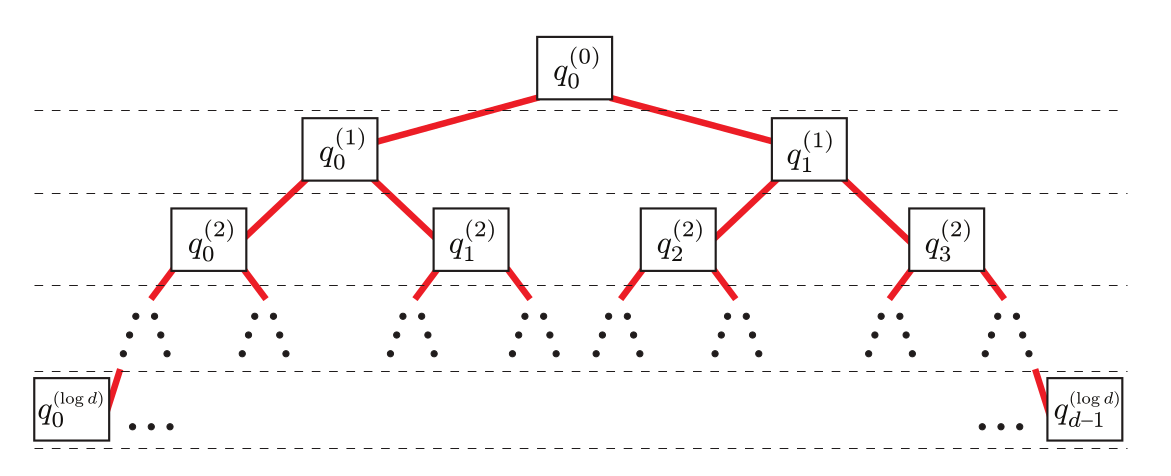
\includegraphics[width=10cm]{Figures/binarytree}
	\caption{Binary tree of region probabilities. The discretised probability for the $i$-th region of $m$-th level is noted $q^{(m)}_i$. Here, $d=N=2^n$.}
\end{figure}

\paragraph{Creating the evolution (\ref{eq:evo}).}
Let us define $x^i_L$ and $x^i_R$ as the left and right boundaries of region $i$, respectively. Define also $x^i_M:=(x^i_R-x^i_L)/2$ and the function
\begin{equation}
	f(i):=\dfrac{\int_{x^i_L}^{x^i_M}p(x)dx}{\int_{x^i_L}^{x^i_R}p(x)dx},
\end{equation}
which represents the probability that $x$ lies in the left half of region $i$.

The critical step of the method, where the challenge resides, is to construct a circuit that efficiently performs the computation
\begin{equation}
	\sqrt{p_i^{(m)}}|i\rangle|0\cdots 0\rangle \rightarrow 	\sqrt{p_i^{(m)}}|i\rangle|\theta_i\rangle,
\end{equation}
where $\theta_i:=\sqrt{f(i)}$. Then, a controlled rotation of $\theta_i$ on the $m+1$-th qubit allows us to obtain
\begin{equation}
	\sqrt{p_i^{(m)}}|i\rangle|\theta_i\rangle|0\rangle \rightarrow \sqrt{p_i^{(m)}}|i\rangle|\theta_i\rangle(\cos\theta_i|0\rangle + \sin\theta_i|1\rangle),
\end{equation}
which can be identified with Equation (\ref{eq:evo}), up to uncomputing $|\theta_i\rangle$.

\subsection{Proposed implementation}

In the following we describe an implementation of the aforementioned procedure, based on \cite{chiang}. Consider Figure \ref{fig:binary-tree} and the notation $q_i:=p_i$ for the discretised version of the probability distribution $p(x)$, we assume to have already calculated. We then have
\begin{equation}
	q_i^{(k-1)} = q_{2i}^{(k)} + q_{2i+1}^{(k)}
\end{equation}
for $k=1,\dots,n$ and $i=0,\dots,2^{k}-1$. The final value is $q_0^{(0)}=1$, i.e., the sum of all probabilities. Initially, the state is
$$
|\psi_0\rangle = |0\rangle_1 |0\rangle_2 \cdots |0\rangle_n.
$$

In the first iteration, the goal is to prepare the state
$$
|\psi_1\rangle = \left(\sqrt{q_0^{(1)}}|0\rangle_0 + \sqrt{q_1^{(1)}}|0\rangle_1\right)|0\rangle_2 \cdots |0\rangle_n
$$
which is achieved by applying the transformation $R(\theta)|0\rangle_1$, where
$$
R(\theta) = \begin{pmatrix}
\cos\theta & -\sin\theta \\
\sin\theta & \cos\theta
\end{pmatrix}
$$
is the rotation transform by an angle $\theta_0^{(1)}=\arccos\sqrt{q_0^{(1)}}$.

After that we generalise for the following iterations: for the $j$-th iteration ($j=2,\dots,n$), the qubits $j$ and higher are still in state $|0\rangle$. So we apply a rotation to the $j$-th qubit of an angle
\begin{equation} \label{eq:theta}
	\theta_i^{(j)}=\arccos\sqrt{\frac{q_{2i}^{(j)}}{q_i^{(j-1)}}}
\end{equation}
depending on the state $|i\rangle$ if the first $j-1$ qubits.

As we already stated, the critical step is to compute the value of the angle $\theta_i^{(j)}$ to apply the rotation. The authors of \cite{chiang} propose the following scheme.

The Determine Angle Circuit (DAC) block computes the state equivalent to the angle $|\theta\rangle$ from the information $|q_{2i}^{(k)}\rangle$ and $|q_{i}^{(k-1)}\rangle$ (as in Equation \ref{eq:theta}), while handling some special cases, namely when $\theta=0$ or $\theta=\pi/2$ (Figure \ref{fig:dac-circuit}).

\begin{figure}[h!]
	\centering
	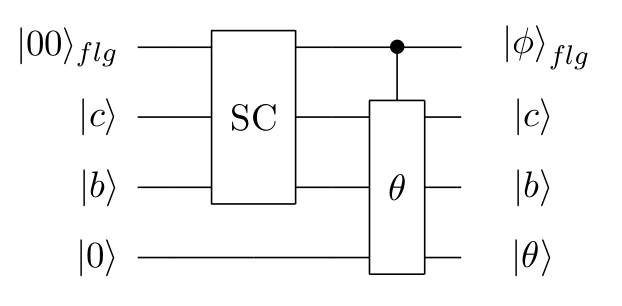
\includegraphics[width=6cm]{Figures/dac-circuit}
	\caption{DAC circuit \cite{chiang}.}
	\label{fig:dac-circuit}
\end{figure}

In the figure, $b=q_i^{(k-1)}$ and $c=q_{2i}^{(k)}$. Special cases are treated by SC circuit block according to Table \ref{tab:sc}.

\begin{table}[h!]
	\centering
	\caption{Special cases treatment.}
	\begin{tabular}{|c|c|}
		\hline
		Flag   & Action               \\ \hline
		00     & compute $\theta$     \\ 
		01, 11 & $\theta=0$ ($b=c$)     \\ 
		10     & $\theta=\pi/2$ ($c=0$) \\ \hline
	\end{tabular}
	\label{tab:sc}
\end{table}

To perform those tests, the block SC is composed by two sub-blocks EQ, which merely tests whether two qubits are the same or not, outputting a flag that indicates the result (Figure \ref{fig:sc-circuit}).

\begin{figure}[h!]
	\centering
	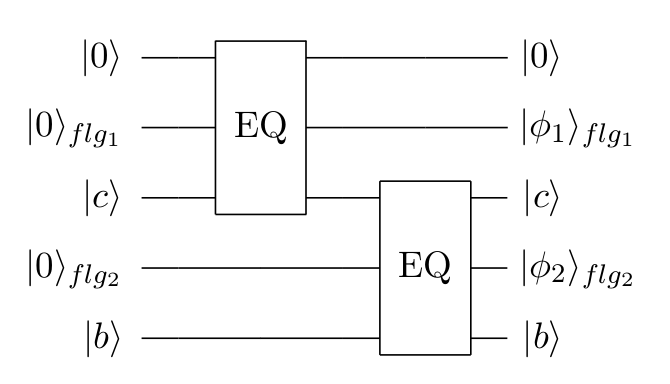
\includegraphics[width=6cm]{Figures/sc-circuit}
	\caption{SC circuit \cite{chiang}.}
	\label{fig:sc-circuit}
\end{figure}

\paragraph{Calculating $\theta$.}
The problem is that, so far, no circuit was proposed to the critical step, which is calculating the angles $\theta_i$ (Equation \ref{eq:theta}, sub-block $\mathrm{\theta}$ in Figure \ref{fig:dac-circuit}). This operation is specially difficult because it involves calculating a division, a square root and an arc-cosine.

The first two operations are addressed in the literature \cite{gokhale, hadfield}. For example \cite{hadfield} presents a method based on a two-stage Newton iteration. Suppose we want to compute $\sqrt{w}$: the first step computes $\hat{x}_{s1}\approx 1/w$, and then the second computes $\hat{y}_{s2}\approx1/\sqrt{\hat{x}_{s1}}\approx\sqrt{w}$ (Figure \ref{fig:sqrt}). While it is not our objective to detail such implementations, we invite the reader to further explore the original document. Henceforth we will simply use the fact that there exists a quantum circuit that compute the square root.

\begin{figure}[h!]
	\centering
	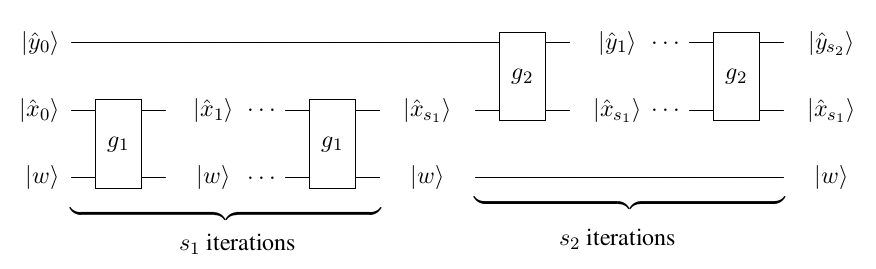
\includegraphics[width=10cm]{Figures/square-root}
	\caption{Circuit to calculate square root \cite{hadfield}.}
	\label{fig:sqrt}
\end{figure}

The most challenging part in the computation of $\theta$ (or at least the one that is not present in the literature, as far as we know) is the arc-cosine computation. Thus we propose a method to obtain using the polynomial series of arc-sine function
\begin{equation}
\arcsin(x) = x +\frac{x^3}{6} + O(x^4)
\end{equation}
and a trigonometric relationship between arc-sine and arc-cosine:
\begin{equation}
	\arcsin(x) + \arccos(x) = \frac{\pi}{2}.
\end{equation}

The circuit that implements the calculus of arc-sine polynomial approximation up to order 3 is presented in Figure \ref{fig:arcsin}.

\begin{figure}[h!]
	\centering
	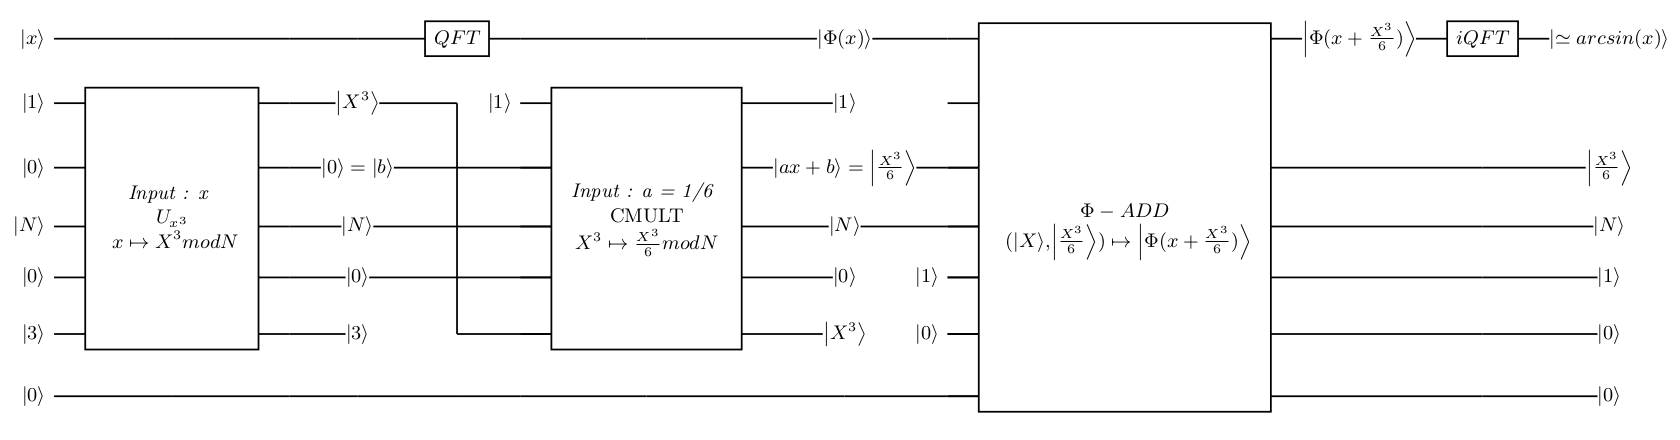
\includegraphics[width=12cm]{Figures/arcsin.png}
	\caption{Circuit to calculate an approximation of $\arcsin(x)$.}
	\label{fig:arcsin}
\end{figure}

\subsection{Discussion}

\paragraph{Complexity.}
An empirical complexity analysis is performed on the approximate arc-sine circuit, considering that this circuit is formed by blocks exponentiation, controlled multiplier, modular adder and QFT (Figure \ref{fig:arcsin}).

From the analysis in \S \ref{sec:complexity}, we already know that CMULT$(a)$-mod-$N$ has complexity $O(n^3)$. Modular adder and QFT blocks have at most the same complexity given that they are used to build CMULT$(a)$-mod-$N$. On the other hand, exponentiation is built as a loop that applies $U_a$-gate $n$ times. As $U_a$-gate has complexity $O(n^3)$, exponential must be $O(n^4)$. Thus, the complete block for computing arc-sine must have complexity of order $O(n^4)$.

We used MATLAB to fit data total number of gates in the circuit as function of $n$, the number of qubits in the input (Figure \ref{fig:data-arcsin}) with $n\in\llbracket 3, 9\rrbracket$. Fitting data to a fourth-degree polynomial we get
\begin{equation*}
	4.584\ n^4 + 31.07\ n^3 -99.99\ n^2 + 605.6\ n - 790.1.
\end{equation*}

\begin{figure}[h!]
	\centering
	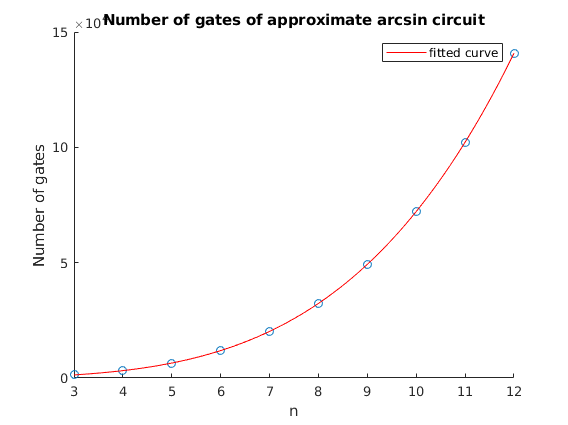
\includegraphics[width=7cm]{Figures/data-arcsin}
	\caption{Circuit to calculate an approximation of $\arcsin(x)$. Drawn with Quantikz \cite{quantikz}.}
	\label{fig:data-arcsin}
\end{figure}

Indeed, this is promising news for our implementation idea, because the final circuit may then be polynomial complex, i.e., there may be an efficient implementation for a circuit that solves the initial problem of creating superpositions that correspond to probability densities.

\paragraph{Representation.}

So far our measured qubits were binary qubits interpreted as integers. However, now we are interested in real numbers, thus we need a bijection from $\{0,1\}^{n}$ (set of infinite list of 0 and 1) to [0,1]. The dyadic development is such a bijection:
$$f(x)=\sum_{j=1}^\infty \frac{x_j}{2^j},$$
where $x_j \in \{0,1\}$\footnote{Note there should not be a infinite sequence of 1 if we are not representing the number 1.}.

Here we are limited to our qubits register size $\hat{N}$. Thus, our precision in $[0,1]$ is $1/2^{\hat{N}}$ and our bijection is now
$$f(x) =\sum_{j=1}^{\hat{N}} \frac{x_j}{2^j}.$$

Our bijection $f$ should have some nice properties such as $f(x\times y) = f(x)\times f(y)$. However, as our number of qubits is finite, we encounter overflows issues. For example, for
$$x = y = \frac{1}{2^{\hat{N}}},$$
$$x \times y = \frac{1}{2^{(1+ \hat{N})}}$$
is outside the definition set of $f$.

We managed to simulate quantum circuit with only 4 or 5 qubits. In our attempt to create an $\arcsin$ gate, we used the approximation $x + \frac{x^{3}}{6}$. Even with our biggest input $x = \frac{1}{2}$ we cannot correctly represent the $\frac{x^{3}}{6}$ term, since $\frac{x^{3}}{6}< \frac{x^{3}}{4} = \frac{1}{2^5}$ (our smallest number).

\clearpage
\newpage
\section{Final considerations}

In this work, we have studied two quantum algorithm: the well-known Shor's algorithm and one for the problem of creating quantum superpositions that correspond to a probability distribution. We were able to implement the former in ProjectQ framework using Python language and to perform factorisation of small numbers (say, 21). For the latter, we propose an implementation based on previous literature, but with the advantage of explicitly presenting a solution to a whole that was left, namely the circuit that computes the angle $\theta$. This circuit has polynomial complexity, which indicates that the whole circuit may be efficient enough to solve the initial problem.

Through this implementation, the basics and principles of quantum computation are presented. This also supports the importance of this new technology for the future of computer science and the incredible improvements it brings to calculations and problem solving.

However, the limitations of classical computers for simulating prevent us from doing costly operations on a high number of qubits. Although some primary quantum computers have been developed, we do not yet have a concrete example of a completely functional one, due to the difficulties of mastering the creation of qubits and controlling quantum properties.

A lot of investments are being dedicated to the buildup of quantum computing and the improvements rates are of the charts. Major companies claim to being close to introducing the first fully-working quantum computer in the near future.

%\newpage
%\begin{appendices}
%\section{Python codes}
%\label{sec:ap}

%This section presents the Pyhton codes with ProjectQ library used to implement Shor's algorithm. Each circuit block described in \S \ref{sec:oracle} is implemented as a separate file.

%\lstinputlisting[language=Python, frame=single, caption={adder}]{../homemade_code/adder.py}

%\lstinputlisting[language=Python, frame=single, caption={modularAdder}]{../homemade_code/modularAdder.py}

%\lstinputlisting[language=Python, frame=single, caption={phi\_adder}]{../homemade_code/phi_adder.py}

%\lstinputlisting[language=Python, frame=single, caption={inv\_phi\_adder}]{../homemade_code/inv_phi_adder.py}

%\lstinputlisting[language=Python, frame=single, caption={cMultModN\_non\_Dagger}]{../homemade_code/cMultModN_non_Dagger.py}

%\lstinputlisting[language=Python, frame=single, caption={inv\_cMultModN\_non\_Dagger}]{../homemade_code/inv_cMultModN_non_Dagger.py}

%\lstinputlisting[language=Python, frame=single, caption={gateUa}]{../homemade_code/gateUa.py}

%\lstinputlisting[language=Python, frame=single, caption={qft}]{../homemade_code/qft.py}

%\lstinputlisting[language=Python, frame=single, caption={iqft}]{../homemade_code/iqft.py}

%\lstinputlisting[language=Python, frame=single, caption={initialisation}]{../homemade_code/initialisation.py}

%\lstinputlisting[language=Python, frame=single, caption={shor}]{../homemade_code/shor.py}

%\lstinputlisting[language=Python, frame=single, caption={shor3n.}]{../homemade_code/shor_3n.py}
	
%\end{appendices}

\clearpage
\newpage
\begin{thebibliography}{10}
	
\bibitem{medium} Braun, Markus C. ``A brief history of quantum computing''. \textit{Medium}. Available in: \url{https://medium.com/@markus.c.braun/a-brief-history-of-quantum-computing-a5babea5d0bd}. Access on: 12 jun. 2019.

\bibitem{shor} Shor, Peter. ``Polynomial-Time Algorithms for Prime Factorization and Discrete Logarithms on a Quantum Computer''. \textit{SIAM Journal on Computing}, vol. 26, no. 5, pp. 1484-1509, 1997.

\bibitem{git} GitHub. \textit{quantum-calculus}. Available in: \url{https://github.com/miyamotohk/quantum-calculus}. Access on: 11 jun. 2019.

\bibitem{valiron} Valiron, B. ``Quantum computation: a tutorial''. \textit{New Generation Computing}, vol. 30, no. 4, pp. 271-296, oct. 2012.

\bibitem{portugal} Portugal, R. et al. \textit{Uma introdu��o � computa��o qu�ntica}. S�o Carlos: SBMAC, 2004.

\bibitem{nielsen} Nielsen, Michael A. and Chuang, Isaac L. \textit{Quantum computation and quantum information}. 10th anniversary edition. Cambridge: Cambridge University Press, 2010.

\bibitem{ekert} Ekert, A. and Jozsa, R. ``Quantum computation and Shor's factoring algorithm''. \textit{Reviews of Modern Physics}, vol. 68, no. 3, pp. 733-753, 1996.

\bibitem{griffighs} Griffiths, Robert B. and Niu, Chi-Sheng. ``Semiclassical Fourier Transform for Quantum Computation''. \textit{Physycal Review Letters}, vol. 76, no. 17, pp. 3228-3231, 1996.

\bibitem{wiki} Wikipedia. \textit{Quantum Fourier transform}. Available in: \url{https://en.wikipedia.org/wiki/Quantum_Fourier_transform}. Access on: 18 dec. 2018.

\bibitem{hardy} Hardy, G. H. and E. M. Wright. \textit{An introduction to the
theory of numbers}. 6th edition. Oxford : Oxford University Press, 2008.

\bibitem{beauregard} Beauregard, Stephane. ``Circuit for Shor's algorithm using $2n+3$ qubits''. \textit{Quantum Information and Computation}, vol. 3, no. 2 pp. 175-185, 2003.

\bibitem{draper} Draper, Thomas G. \textit{Addition on a quantum computer}. Available in: \url{https://arxiv.org/abs/quant-ph/0008033}. Access on: 14 dec. 2018.

\bibitem{projectq} ProjectQ. Availabe in: \url{https://projectq.ch/}. Access on: 28 nov. 2018.

\bibitem{steiger} Steiger, Damian S.; H�ner, Thomas and Troyer, Matthias. ``ProjectQ: an open source software framework for quantum computing''. \textit{Quantum}, vol. 2, p. 49, jan. 2018.

\bibitem{grover} Grover, L. and Rudolph, T. \textit{Creating superpositions that correspond to efficiently integrable probability distributions}. Available in: \url{https://arxiv.org/abs/quant-ph/0208112}. Access on: 9 may 2019.

\bibitem{chiang} Chiang, Chen-Fu; Nagaj, Daniel; Wocjan, Pawel. ``Efficient Circuits for Quantum Walks''. \textit{Quantum Information \& Computation}, vol. 10, no. 5, pp. 420-434, 2010.

\bibitem{gokhale} Gokhale, Pranav. \textit{Implementation of Square Root Function Using Quantum Circuits}. Princeton University, 2014. Available in: \url{http://www.undergraduatelibrary.org/2014/computer-sciences/implementation-square-root-function-using-quantum-circuits}. Access on: 19 jun. 2019.

\bibitem{hadfield} Hadfield, Stuart Andrew. \textit{Quantum Algorithms for Scientific Computing and Approximate Optimization}. PhD Thesis, Columbia University, 2018. Available in: \url{https://arxiv.org/abs/1805.03265}. Access on: 19 jun. 2019.

\bibitem{quantikz} Kay, Alastair. \textit{Tutorial on the Quantikz Package}. Available in: \url{https://arxiv.org/abs/1809.03842}. Access on: 12 jun. 2019.

\end{thebibliography}

\end{document}
